\newpage
\section*{Interaction Heatmaps}

\begin{figure}[H]
  \caption{Whole Genome Heatmaps}\label{fig:WholeGenomeHeatmaps}
  \begin{minipage}{0.5\textwidth}%
    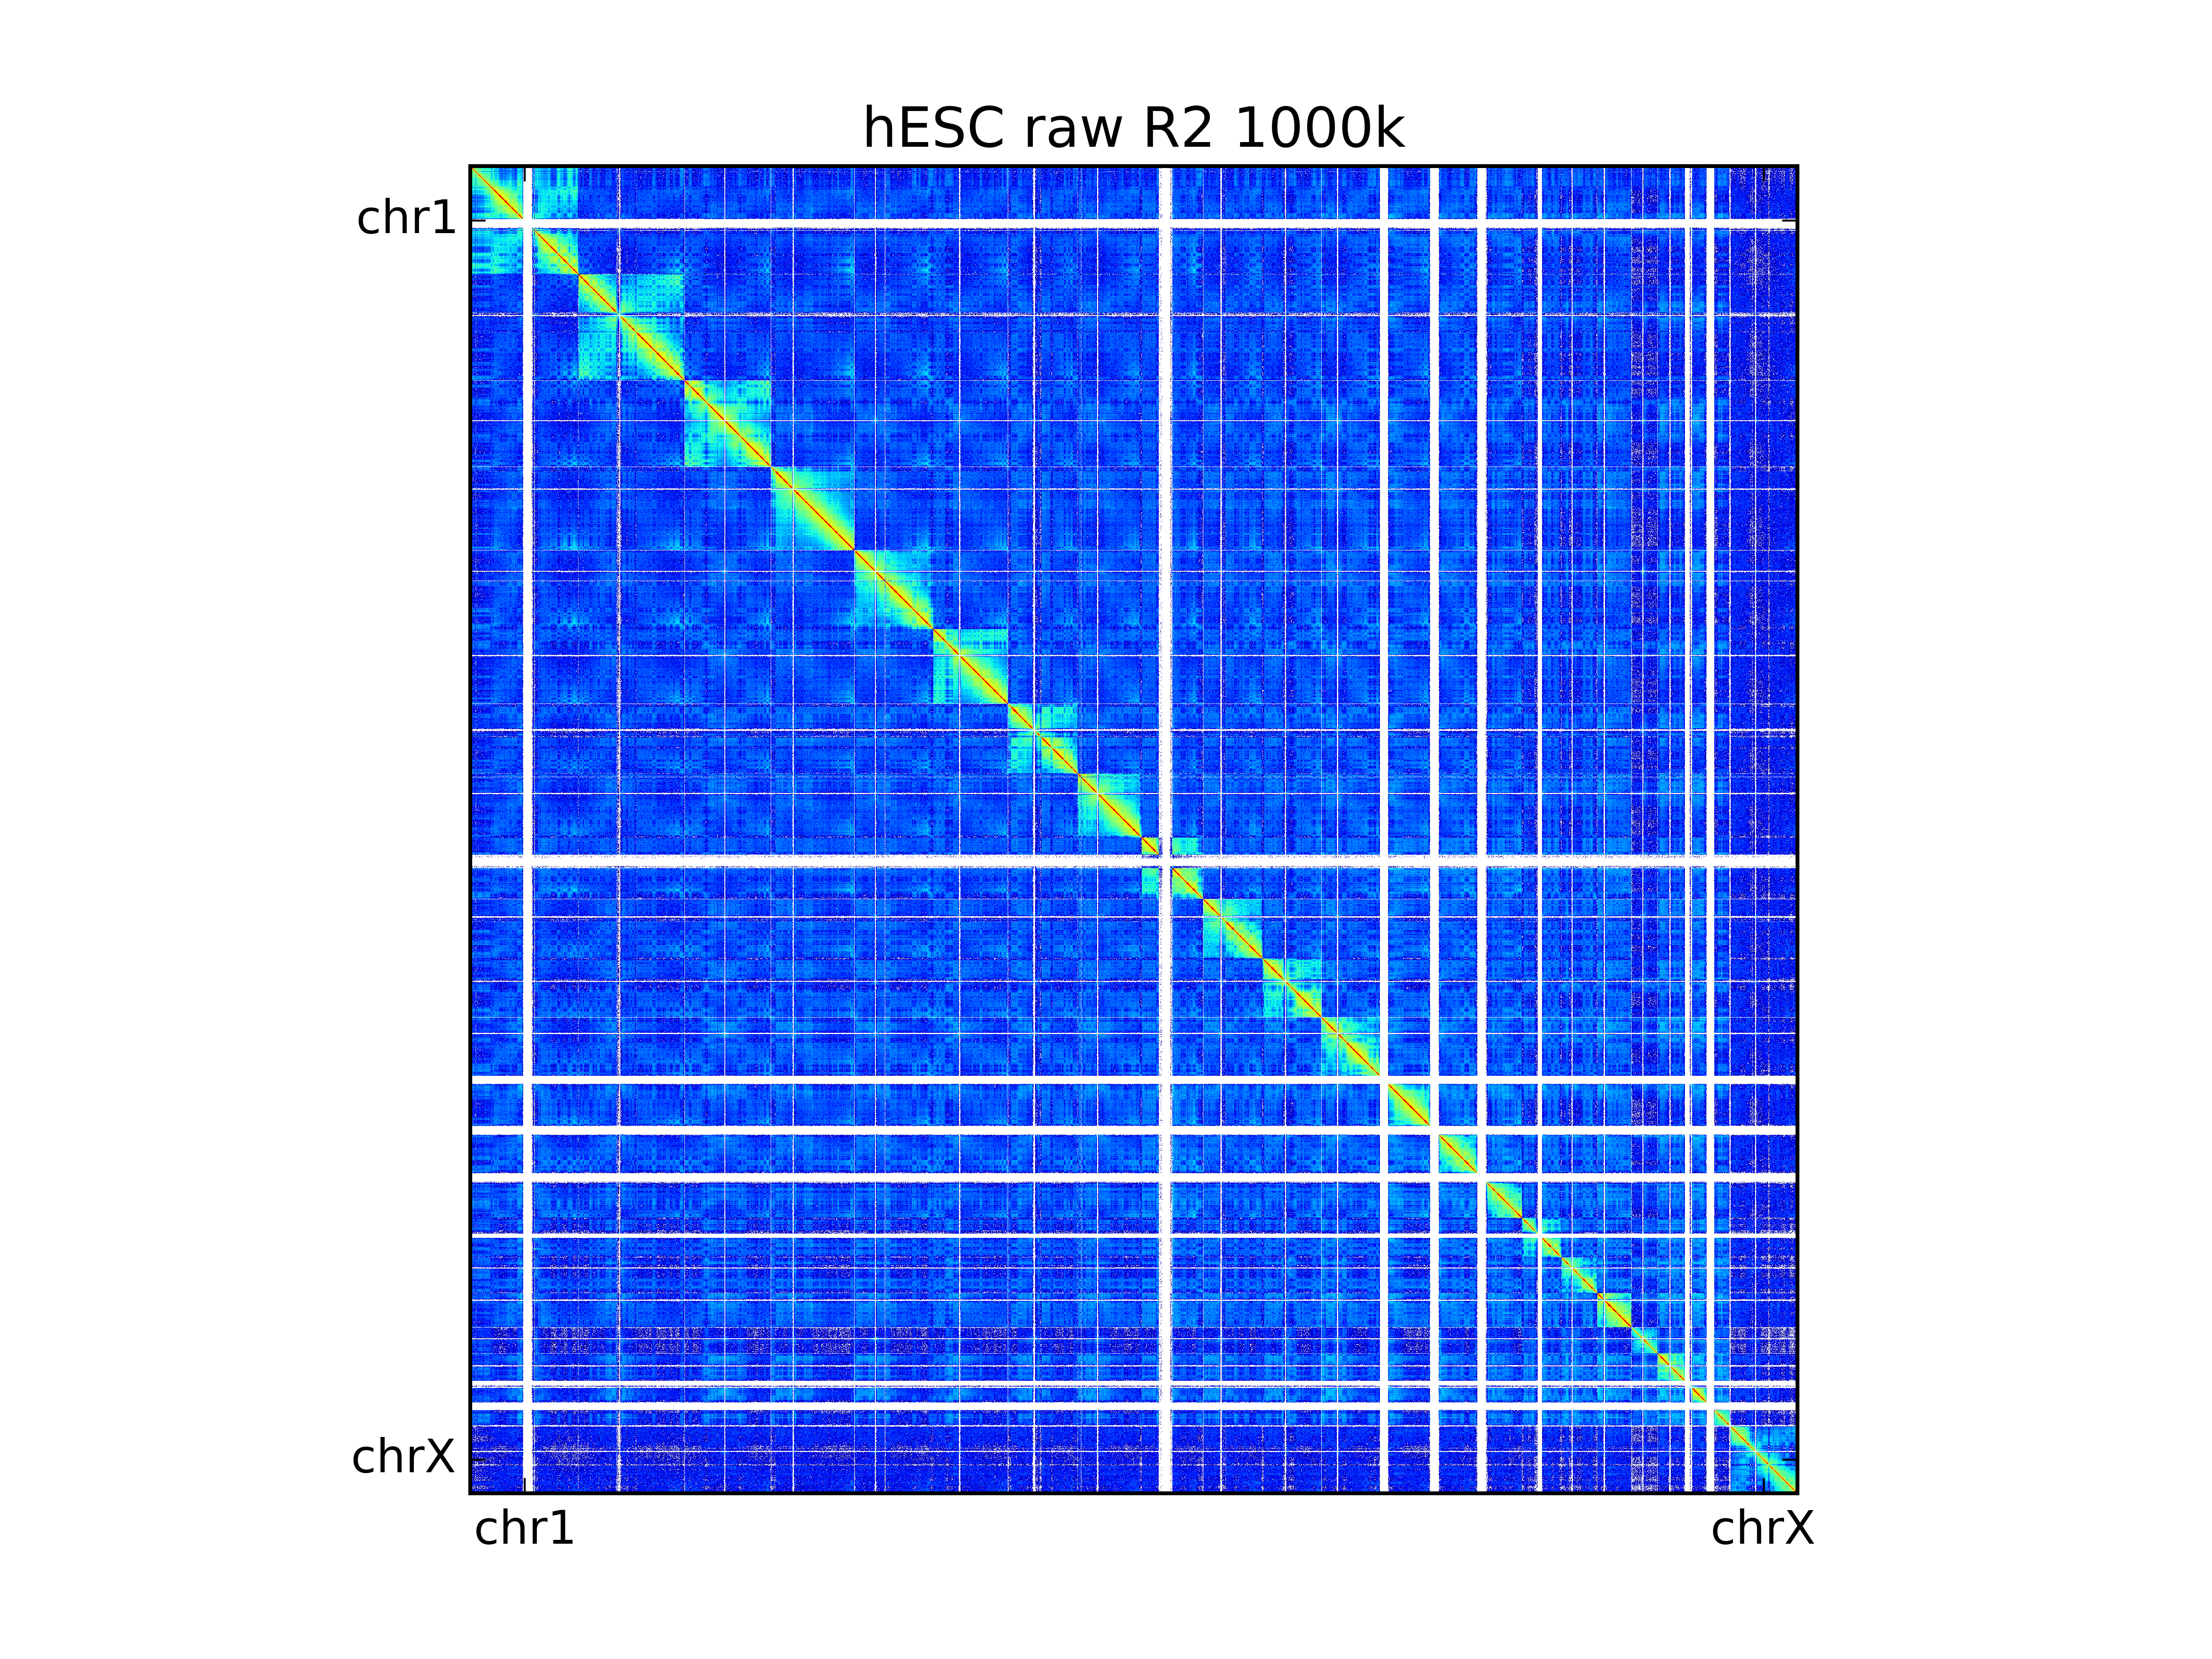
\includegraphics[width=\textwidth]{./figures/supplementary/hm/hesc_raw_1Mb.png}
  \end{minipage}%
  \hfill
  \begin{minipage}{0.5\textwidth}
    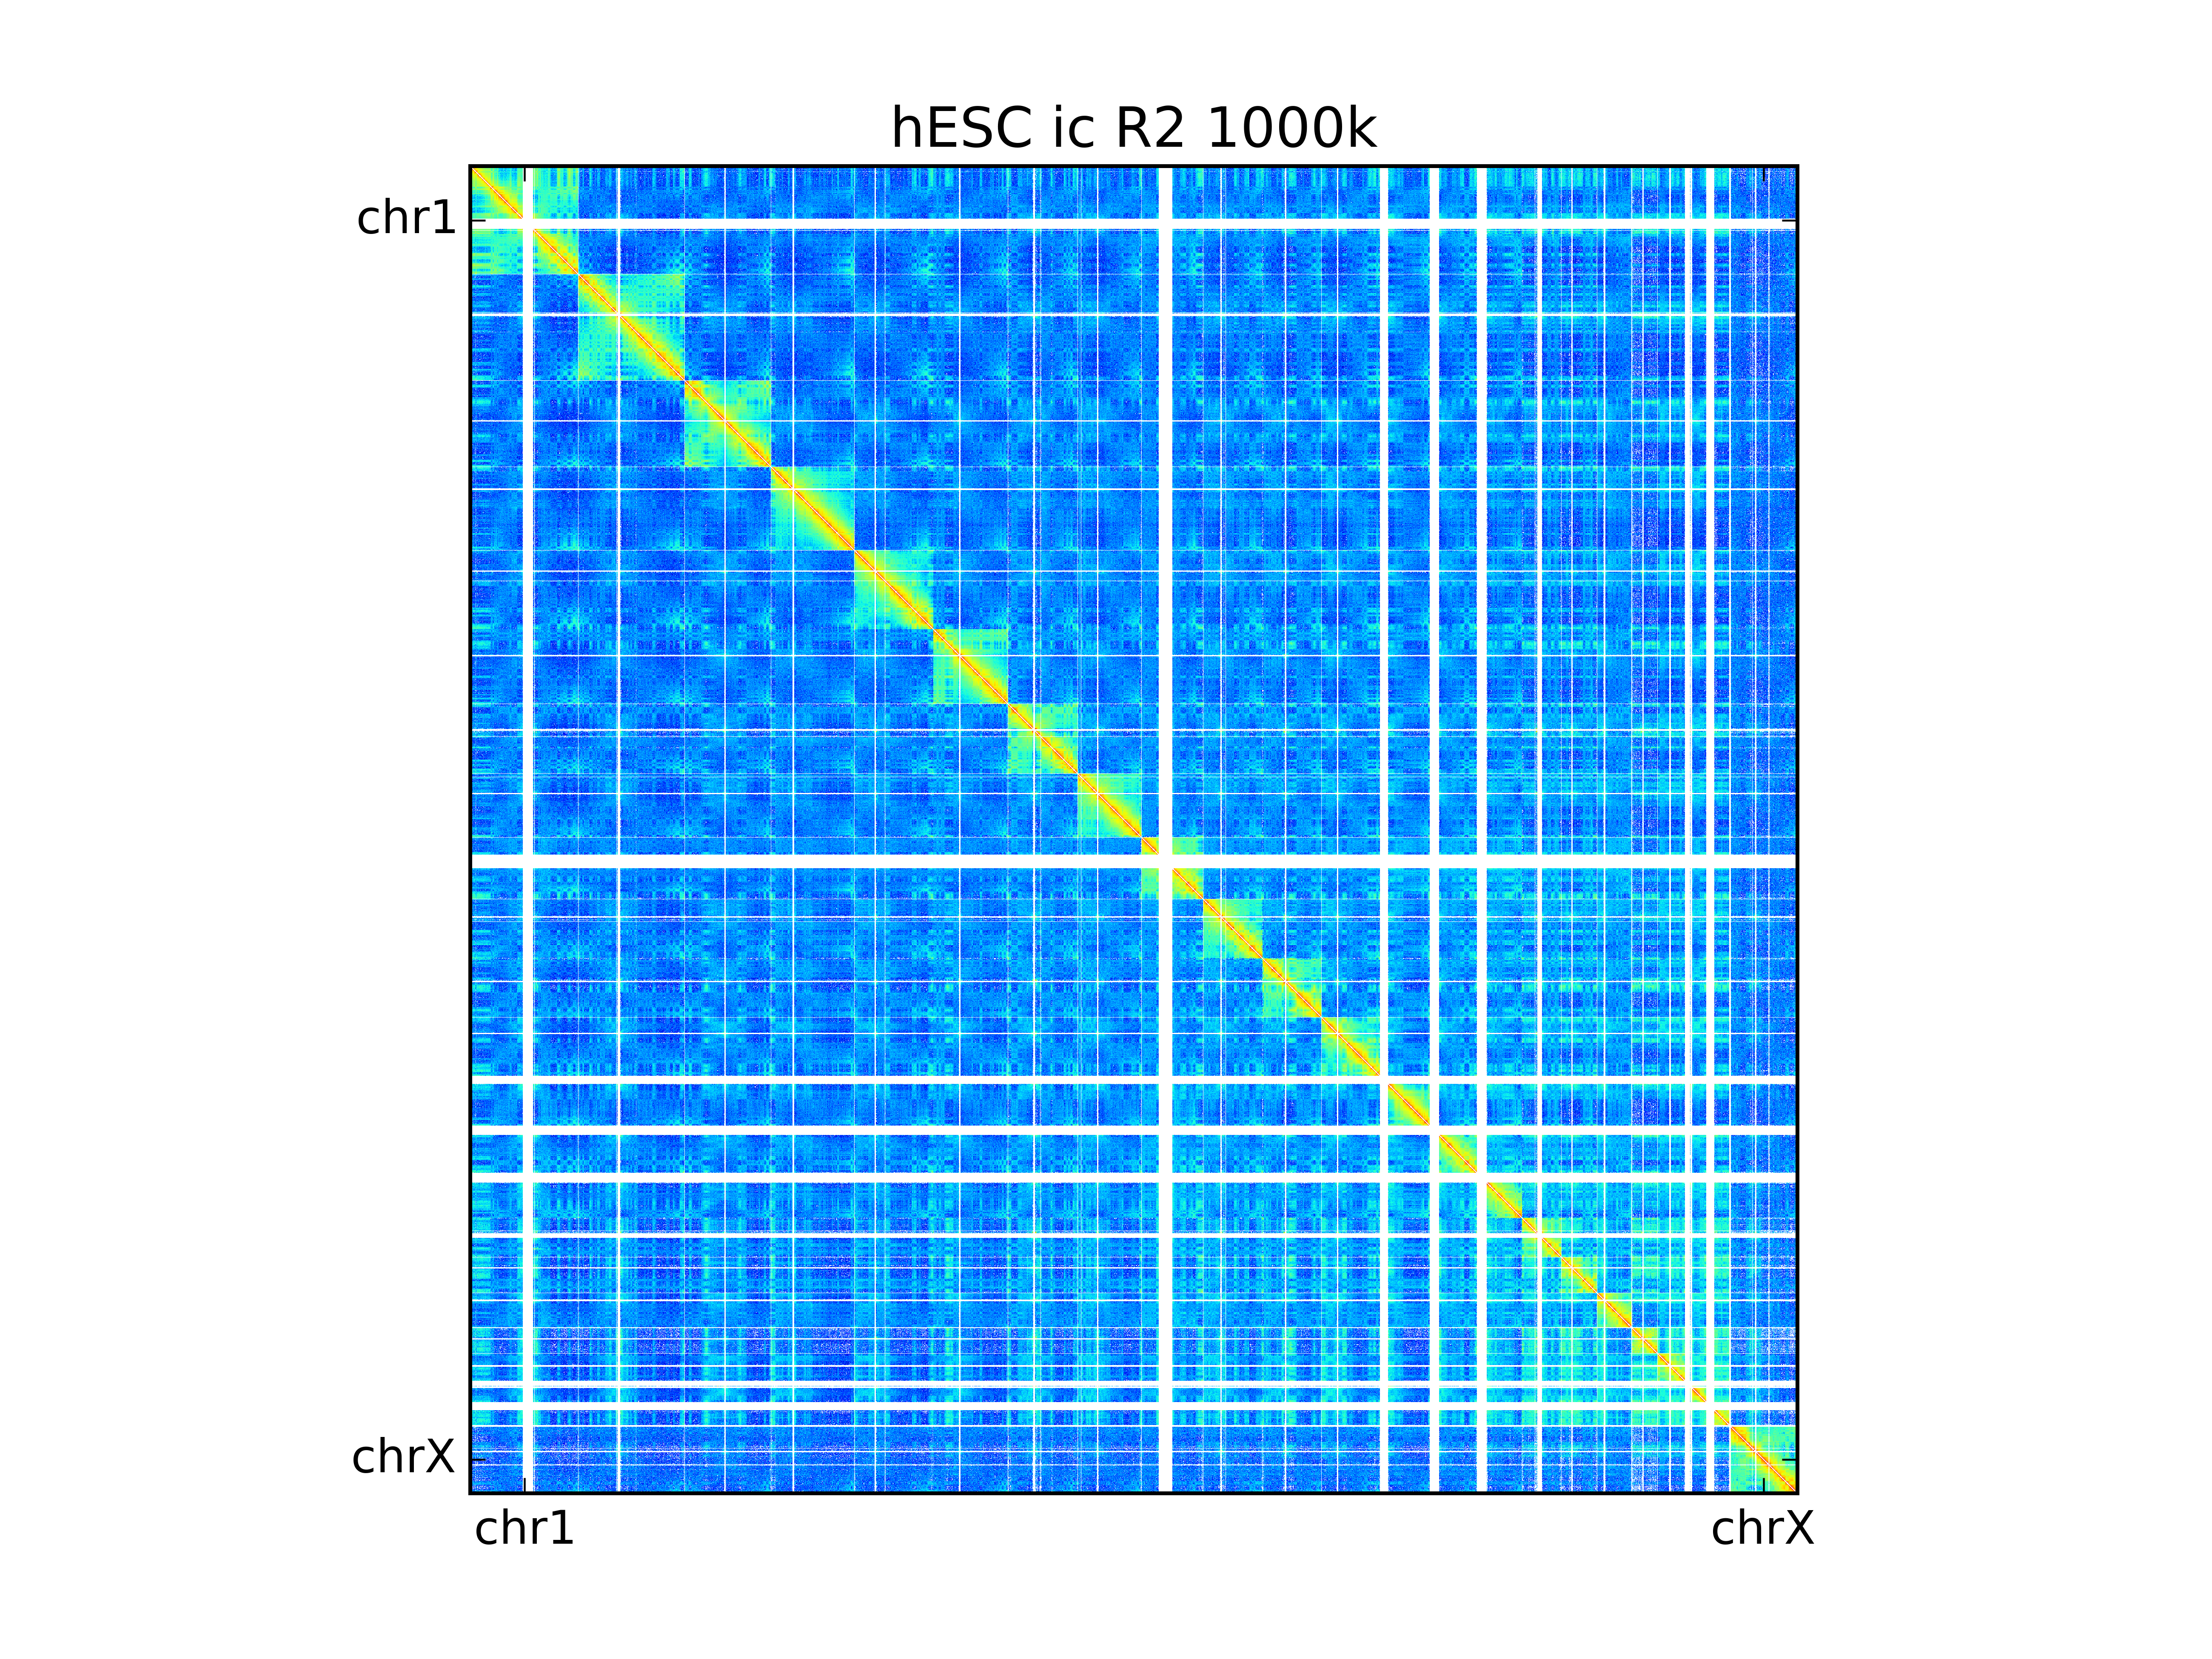
\includegraphics[width=\textwidth]{./figures/supplementary/hm/hesc_ic_1Mb.png}
  \end{minipage}
\end{figure}

\begin{figure}[H]
  \begin{minipage}{0.5\textwidth}%
    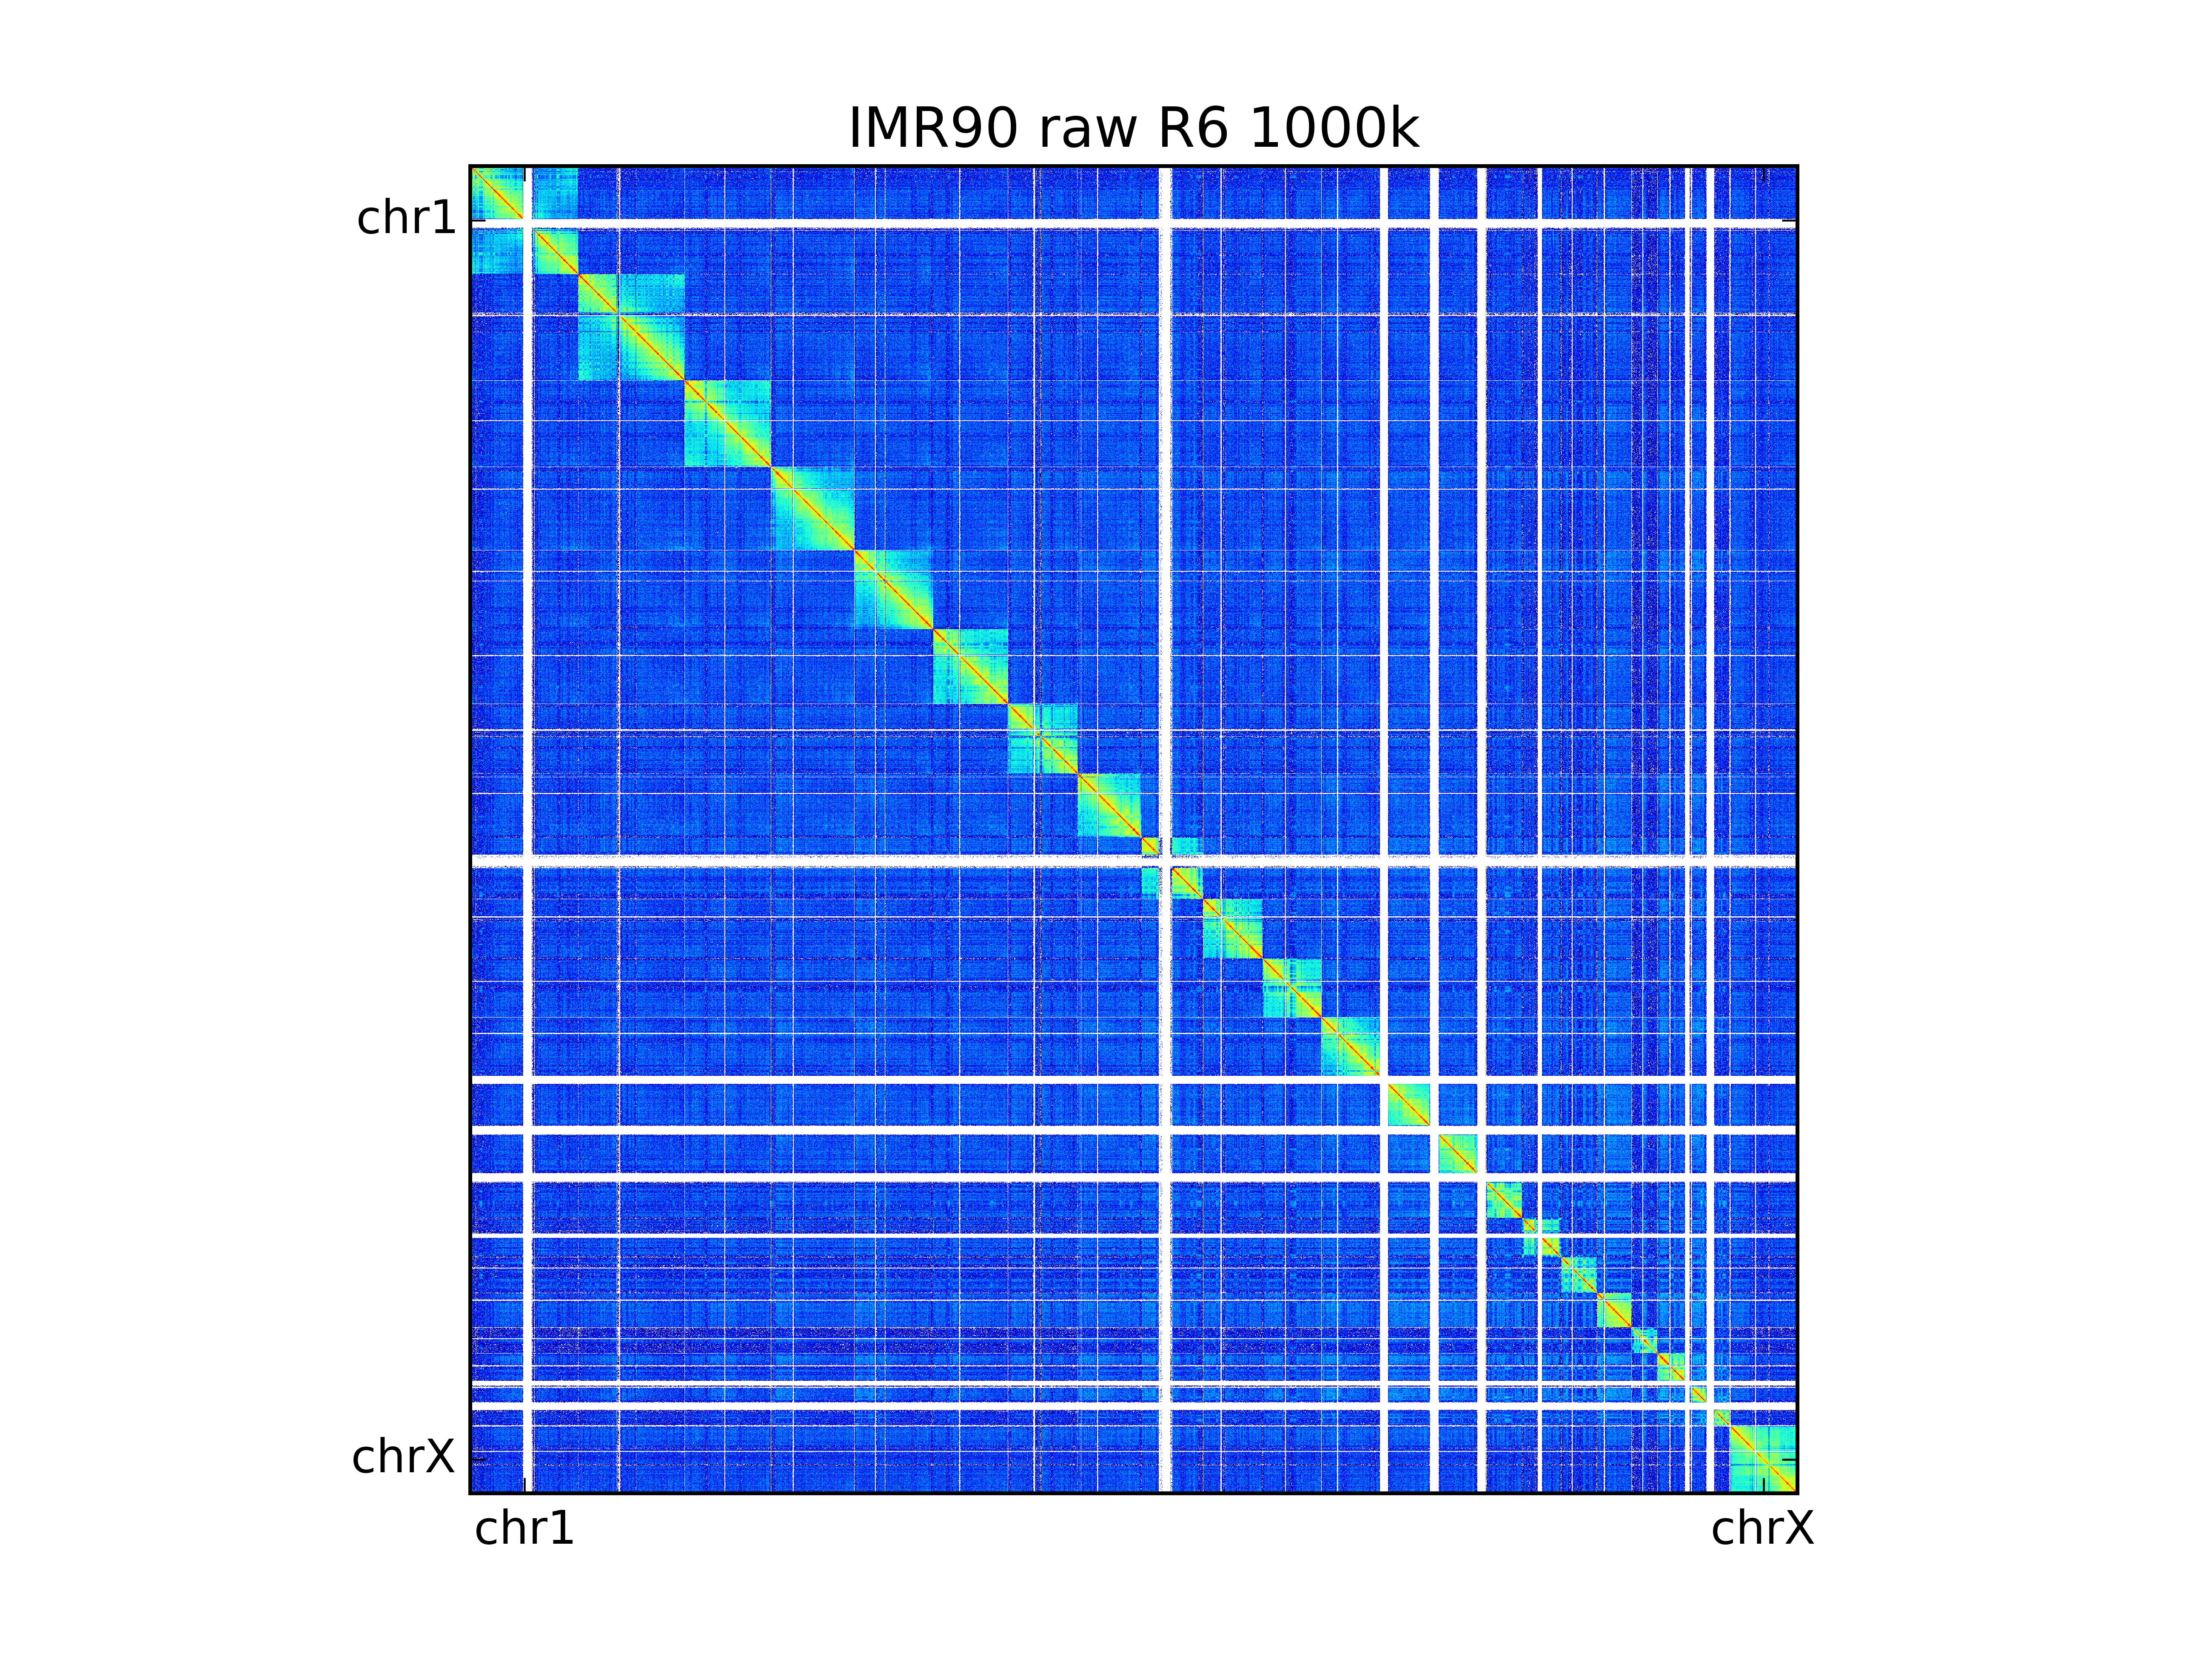
\includegraphics[width=\textwidth]{./figures/supplementary/hm/imr90_raw_1Mb.png}
  \end{minipage}%
  \hfill
  \begin{minipage}{0.5\textwidth}
    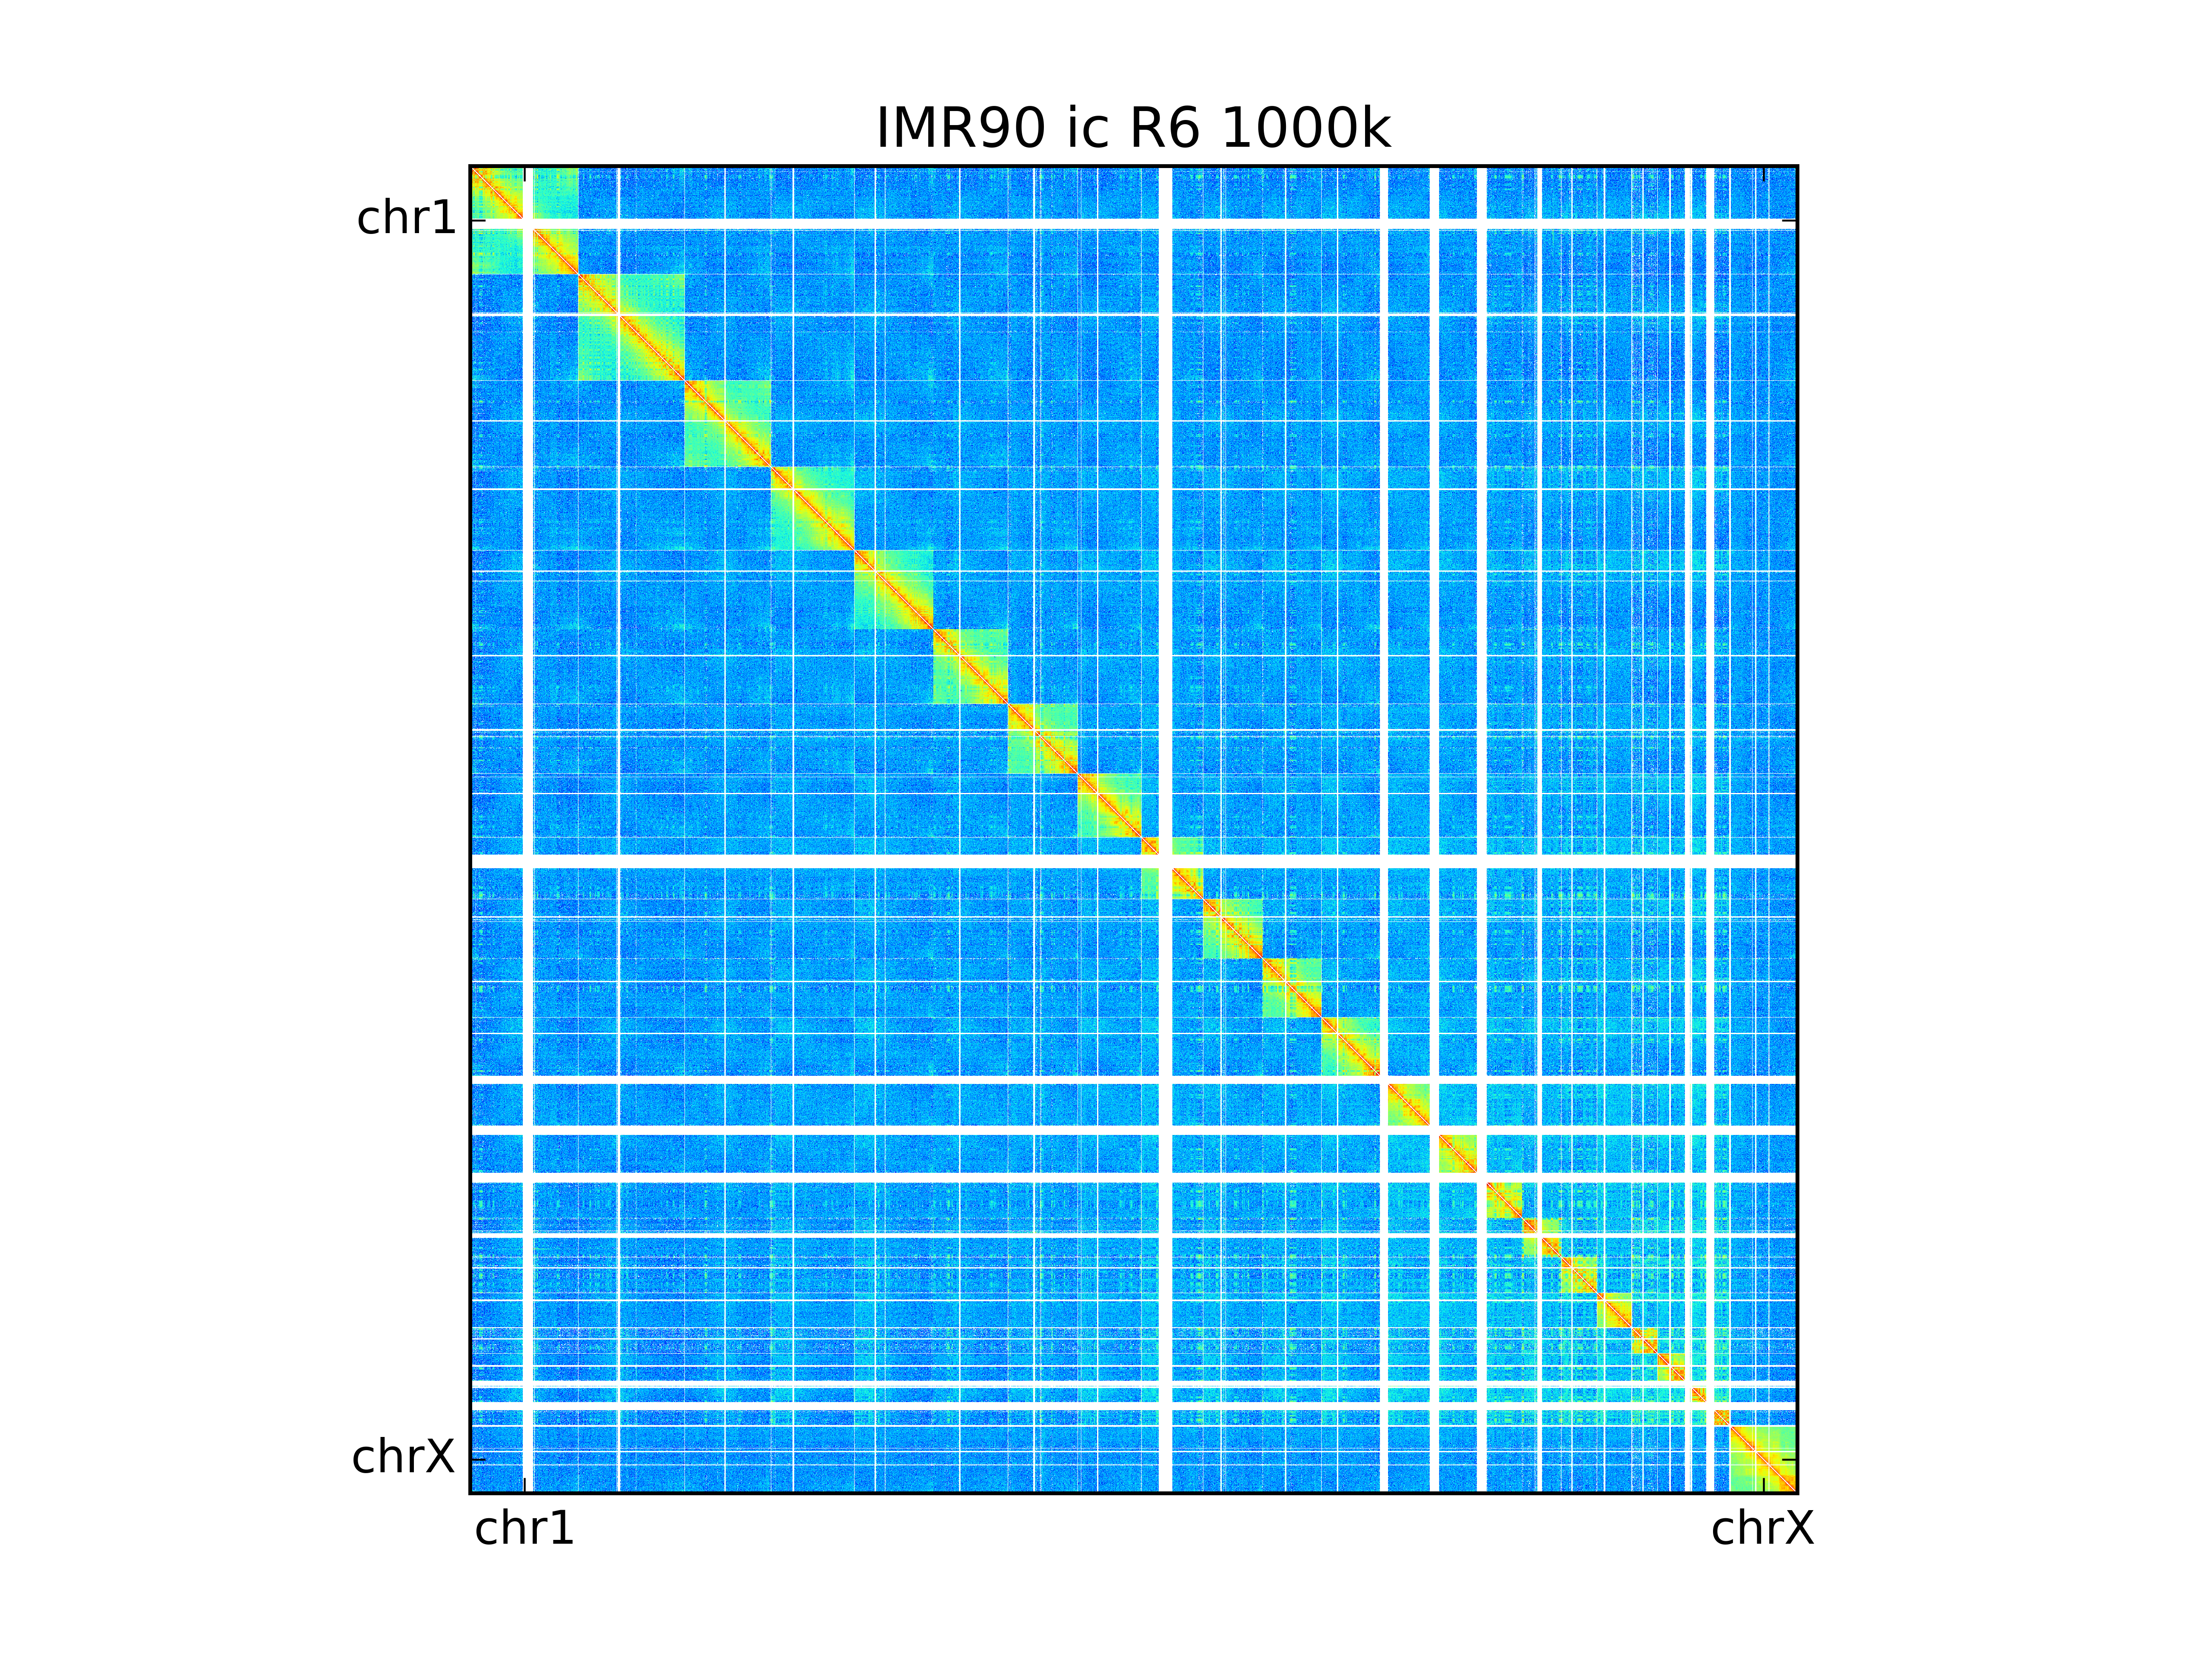
\includegraphics[width=\textwidth]{./figures/supplementary/hm/imr90_ic_1Mb.png}
  \end{minipage}
  \small
  Genome heatmaps constructed from raw (left) and normalized (right) interaction maps.
  Chromosomes are arranged as blocks on the diagonal.  Each light colored block on the
  diagonal shows regions of increased interactions.  White bands correspond to regions
  of noise removed due to noise, typically around centromeres and telomeres.
\end{figure}

\begin{figure}[H]
  \caption{IMR90 Chromosome 2 Banding}\label{fig:Chrom2Banding}
  \begin{minipage}{0.5\textwidth}%
    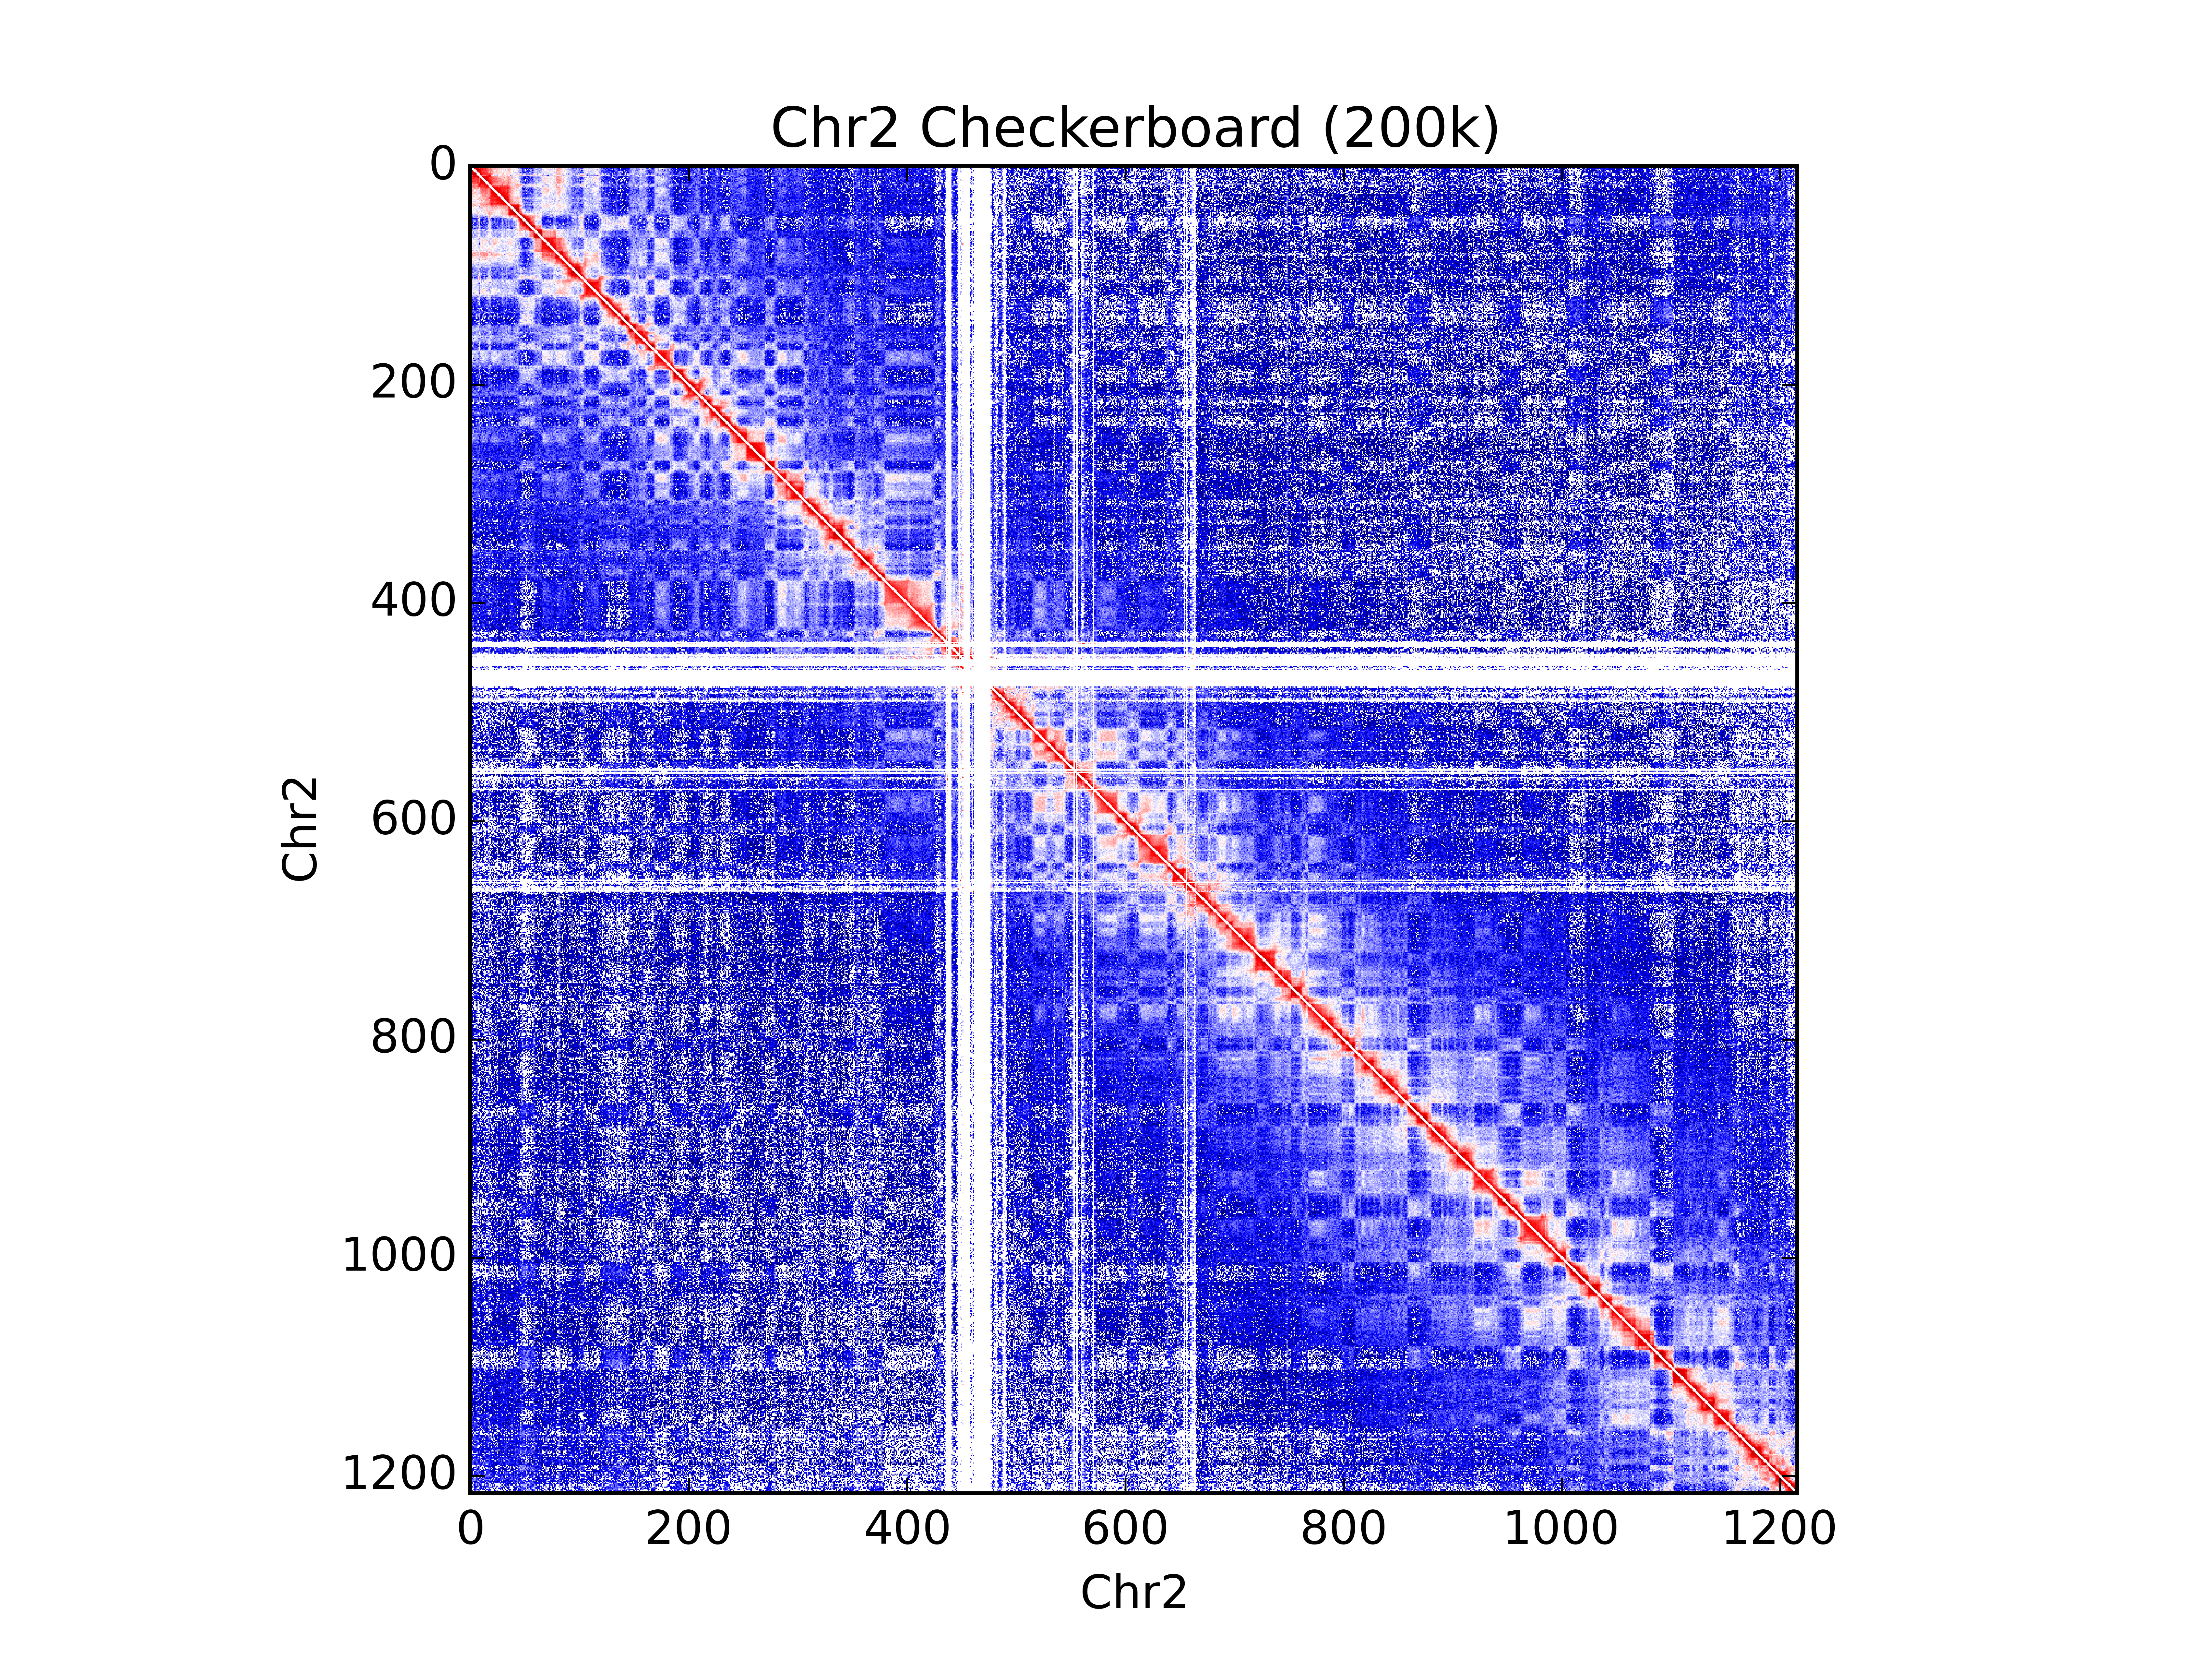
\includegraphics[width=\textwidth]{./figures/supplementary/hm/IMR90-R1-200k-Chr2.png}
  \end{minipage}%
  \hfill
  \begin{minipage}{0.5\textwidth}
    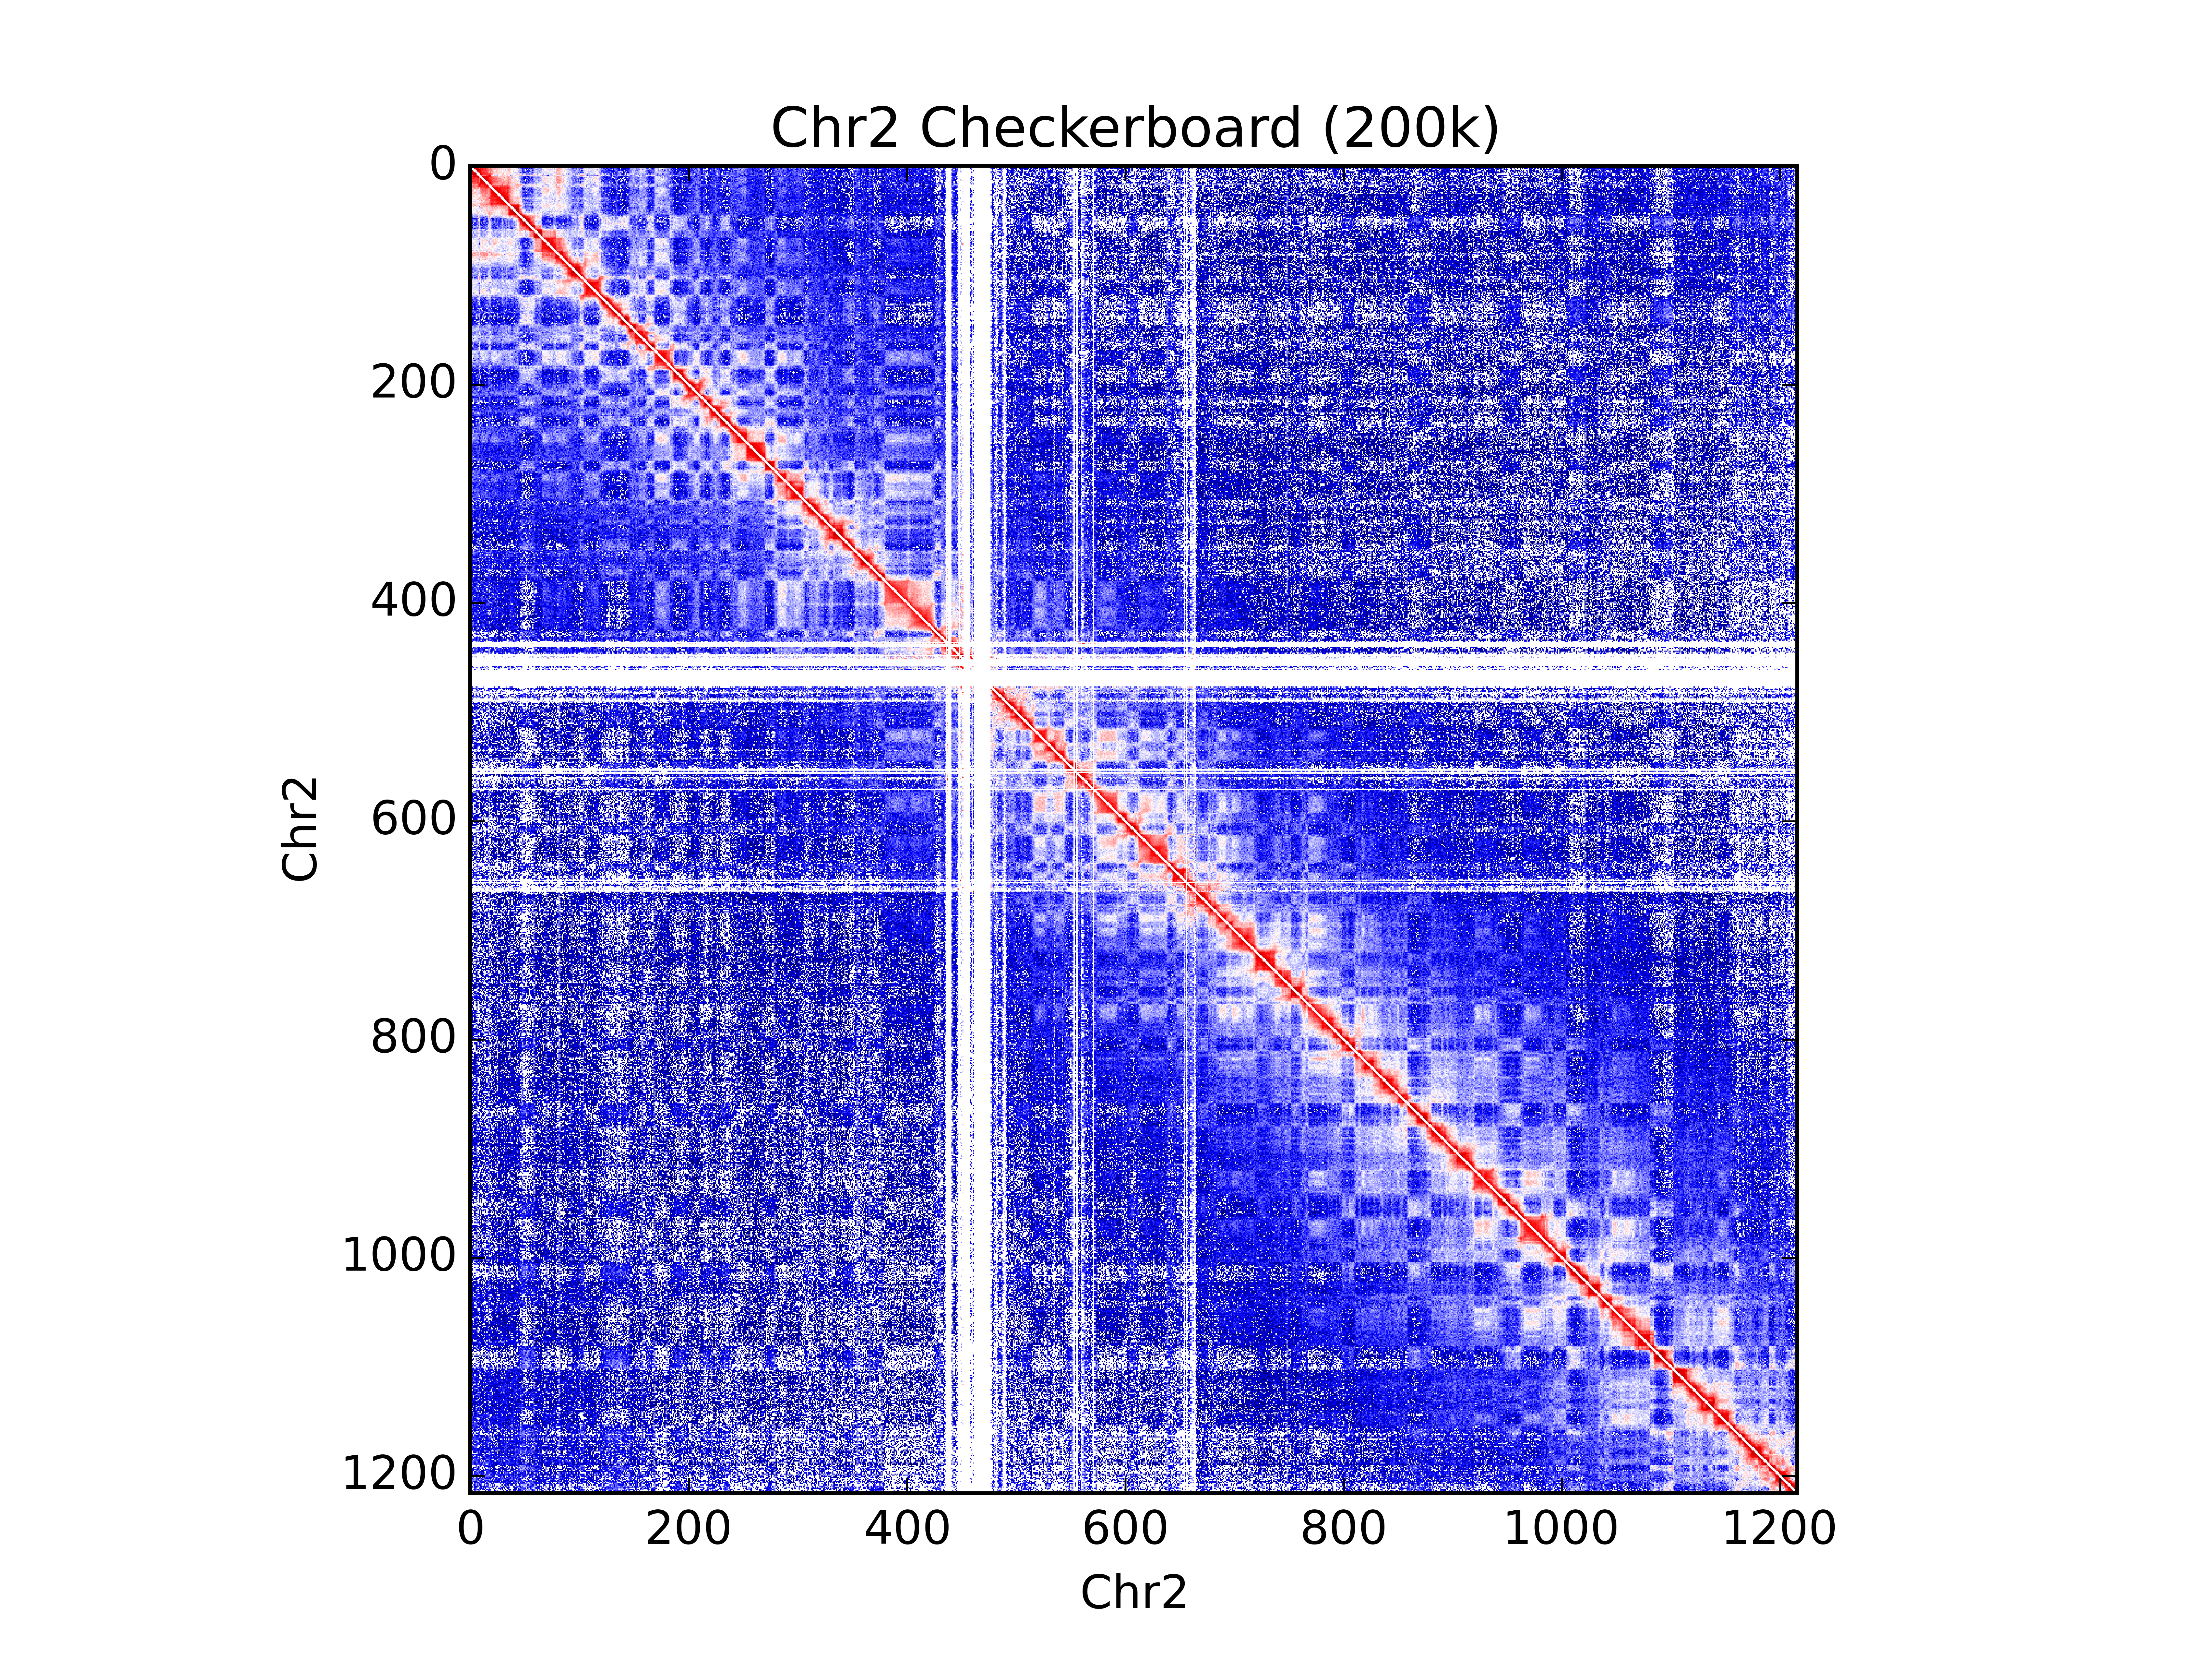
\includegraphics[width=\textwidth]{./figures/supplementary/hm/IMR90-R1-200k-Chr2.png}
  \end{minipage}
  \small
  IMR90 Replicates I and II\@.  The red and blue coloring reveals the banding patterns described by
  \citet{dekker2012}, indicating areas of above average or lower than average interactions.  These chromatin
  compartments are captured in the first two principal components.
\end{figure}


\begin{table}[H]
  \centering
  \caption{Mapping Statistics}\label{tab:hmstats}
  \begin{tabular}{cccc}
    \toprule
    Map & Total Reads & Post-Filtering & Percent \textit{Trans} \\
    \midrule
    hESC R1  & 199955400 & 18295668  & 48.6\% \\
    hESC R2  & 433584106 & 125581108 & 23.6\% \\
    IMR90 R1 & 349117513 & 90481608  & 37.3\% \\
    IMR90 R2 & 398642708 & 157378922 & 50.6\% \\
    IMR90 R3 & 528662422 & 72996792  & 59.9\% \\
    IMR90 R4 & 463140318 & 53109981  & 54.2\% \\
    IMR90 R5 & 203181628 & 41901503  & 46.9\% \\
    IMR90 R6 & 181708889 & 41429368  & 49.0\% \\
    \midrule
    Total & 2757992984 & 601174950 & {} \\
    \bottomrule
  \end{tabular}
\end{table}
